\chapter{Begriffe und Definitionen}
\section{Kontinuierlich und Diskret}
Das zu messende Feld ist in der Regel eine kontinuierliche Funktion von Ort oder Zeit z.B. $x(t)$. Dabei ist $t$ die unabhängige und $x$ die abhängige Variable. Sowohl abhängige wie unabhängige Variablen sind kontinuierlich und können in einem bestimmten Wertebereich stufenlos jeden Wert annehmen. Durch Art der Messung (z.B. punktweise Messung) und Diskretisierung wird eine diskrete Wertereihe erhalten, wobei abhängige und unabhängige Variablen nur bestimmte, mit endlich vielen Ziffern darstellbare Werte annehmen können. Das Resultat ist die diskrete Wertereihe  $\{x_{i}\}=\{x_{1}, x_{2}, x_{3}, \dots, x_N\}$, wobei $t_{i}=i\Delta t$, mit $i=1,2, \dots, N,$ ist, mit einem Abtastschritt $\Delta t$. Nur diskrete Wertereihen sind für die digitale Bearbeitung mit Computern geeignet.  Die Funktion $x(t)=\cos(\omega t)$ ist kontinuierlich bzgl. Zeit und Amplitude, die Wertereihe $\{ x_i \}= \{1,0,-1,0,1,0,-1,0\}$ ist dagegen diskret bzgl. Zeit und Amplitude. Die Spannung am Ausgang eines Seismometers ist kontinuierlich bzgl. Zeit und Amplitude, während die Spannung am Ausgang eines Computers zwar kontinuierlich bzgl. der Zeit ist, mitunter aber nur bestimmte Werte annehmen kann, also diskret bzgl. der Amplitude sein kann. Man muss also eine Diskritisierung bezüglich der Zeit oder bezüglich der Amplitude durchführen um die Messdaten digial bearbeiten zu können.\\

Die Darstellung einer Messgröße kann analog oder digital erfolgen, d.h. in Form einer messbaren physikalischen Größe bzw. in Form von Ziffern. Beispiele für analoge Darstellungen sind graphische Darstellungen auf Bildschirm oder Papier, Seismogrammschriebe, wie sie bis in die 70er Jahre des letzten Jahrhunderts üblich waren oder Aufzeichnungen auf Magnetband.  Die Anzeige der Uhrzeit kann analog oder digital erfolgen.  Die Auflistung von Wertereihen ist dagegen ein Beispiel für die digitale Darstellung. Die Schallplatte ist ein analoger Datenträger, eine CD oder DVD sind digtiale Datenträger. Die digitale Darstellung von Diskreten Zahlen kann mittels Binärzahlen zur Basis 2 erfolgen. Beispiel der ganzen Zahl 11 als Binärzahl 1011,
\[
11 = \mathrm{bin}(1011) =1\cdot 2^{3} + 0 \cdot 2^2 + 1 \cdot 2^1 + 1 \cdot 2^0 =11.
\]
Um einen großen Wertebereich mit wenigen Bits darzustellen, kann eine Verstärkung definiert werden. Ein Beispiel ist die 16-Bit Datenerfassung die für die Darstellung von seismologischen Registrierungen verwendet worden ist. Dazu wurden ein Bit für das Vorzeichen $V$, nur 11 Bits für die binäre Darstellung eines Faktors $F$  und 4 Bits für die binäre Darstellung des Exponent $E$ von 2 benötigt, durch den eine Verstärkung definiert wurde: $2^{E}$. Der dargestellte Wert ergibt sich dann nach
\begin{equation}
x = V\,F\,2^E. 
\end{equation}
So ist im 16-Bit System $F_{min}=0$ und $F_{max}=2^{11}-1 = 2047$. Für $E_{min}=0$und $E_{max}=2^{4}-1=15$ und also ist die maximale Verstärkung $2^{15}$. So ergibt sich für den maximal darstellbaren Wert $x_{max}=(2^{11}-1) \cdot 2^{15} \approx 2^{26}$. Der minimale Wert hat ein negatives Vorzeichen und ist $x_{min} \approx = -2^{26}$.\\
Die Verstärkung muss optimal gewählt werden, um die kleinsten Bodenbewegungen zu registrieren und gleichzeitig auch große Bewegungen darzustellen.

\subsection{Dynamik einer Signals}
Die Dynamik oder auch der Dynamikumfang ist das Verhältnis zwischen maximalem darstellbaren Betrag und minimalem darstellbaren Betrag größer Null. Der Dynamikumfang wird ausgedrückt als
\begin{equation}
20\log \frac{A_{\textrm{max}}}{A_{\textrm{min}}}\,dB\footnote{Die Einheit ist dB und steht für Dezibel. Dieses Kunstwort ist angelehnt an Graham Bell den Erfinder des Telefons.}
\end{equation}
Dabei ist $A_{\textrm{max/min}}$ ist die größte bzw. geringste Amplitude\\
Weiter ist zu bemerken, dass mitunter auch der Vorfaktor 10 verwendet wird.\\

Der Dynamikumfang eines Seismometers hängt von der Bauart ab und unterscheidet sich somit im Apparat. Das Seismometer vom Typ STS2 kann maximale Geschwindigkeiten der Bodenbewegung bis ca. 0.1 m/s registrieren. Die kleinste registrierbare Geschwindigkeit ist ca. 1 nm/s. Es ergibt sich ein Dynamikumfang von ca. 160 dB. Die oben dargestellte 16-Bit Datenerfassung besitzt eine Dynamik von ca. 156 dB, eine Darstellung mittels Binärzahlen und 24 Bit ergibt eine Dynamik von ca. 145 dB. Diese Datenerfassungen können also den Dynamikumfang des Seismometers nahezu abdecken. Offensichtlich muss die Verstärkung vor dem Analog-Digital-Wandler geeignet gewählt werden, so dass der interessierende Amplitudenbereich durch die Datenerfassung digitalisiert werden kann. Bei zu großer Verstärkung werden große Amplituden nicht mehr dargestellt (eng. \textsl{Clipping} oder Sättigung).  Bei zu geringer Verstärkung können kleine Amplituden nicht unterschieden werden. \\

Zum Vergleich können wir die Dynamik eines seismologischen Papierschriebs abschätzen. Der maximale Ausschlag der Nadel könnte 15 cm betragen, der minimal noch wahrnehmbare Ausschlag 1 mm. Daraus ergibt sich eine Dynamik von ca. 43 dB. Da die Dynamik ein logarithmisches Maß ist, wird deutlich, dass für einen Papierschrieb das Verhälnis von maximal zu minimal darstellbarer Amplitude wesentlich kleiner ist als für digitale Datenerfassungen. 
 

\subsection{Signalauflösung} 
Neben der Dynamik ist die Auflösung ein wichtiger Parameter digitaler Darstellungen. Sie beschreibt die minimal darstellbare Differenz zwischen benachbarten darstellbaren Werten $\Delta x$. Für Binärzahlen ist sie 1. Für die besprochene 16-Bit Darstellung ergibt sich: $(x + \Delta x)= V( F\pm 1)\cdot 2^E$. Die Auflösung ist also vom Exponenten abhängig und für größere Verstärkungen ist die Differenz zwischen benachbarten Werten größer. Die darzustellende Messgröße wird dann bei größeren Werten gröber diskretisiert. Generell muss je nach Aufgabenstellung ein Kompromiss zwischen Dynamik und Auflösung gefunden werden, da nur ein bestimmte Anzahl an Bits für die Darstellung eines Wertes zur Verfügung steht. Es muss also überlegt werden, welche Frequenzen die zu beobachtenden Erdbebenwellen haben. Handelt es sich um teleseismische Ereignisse oder steht die Station in der Nähe des Epizentrums, wo die Bodenbeschleunigung bis 2 g erreichen können. Es gibt auch speziellen Seismometer, welche die Bodenbewegung nahe des Epizentrums aufzeichnen können (\textsl{Strong-Motion} Seismometer)

\subsection{Least Significant Bit}
Ist der Faktor, mit dem $x$ multipliziert werden muss, um die Messgröße zu erhalten. Die Datenerfassung liefert zunächst nur einen einheitenlosen diskreten Wert. Erst durch Multiplikation mit dem \textsl{least significant bit} wird die Messgröße dargestellt. Zum Beispiel wird für seismologische Anwendungen das least signifcant Bits einer 24-Bit Datenerfassung oft 1.67 nm/s gewählt. 


\section{Deterministische und Stochastische Modelle}
Um eine Wertereihe bearbeiten zu können, muss zunächst eine mathematische Beschreibung oder ein Modell für die Wertereihe aufgestellt werden. Dabei kann es sich um ein stochastisches oder ein deterministisches Modell handeln.\\

Ein {\bf deterministisches} Modell kann durch digitale Werte oder durch einen funktionalen Zusammenhang beschrieben werden: z.B. $\{x_i\} = \{0,1,1,0,-1,-1,0\}$ oder $\cos(\omega_0t)$. Deterministische Modelle sind meistens vorhersagbar - Z.B. eine harmonische Schwingung $\cos(\omega_0t)$. Jedoch sind chaotische deterministische Systeme nicht vorhersagbar.\\


Ein \textbf{stochastisches Modell} wird mit Hilfe von Wahrscheinlichkeitsdichteverteilungen (eng. \textsl{Propability Density Function}, PDF) beschrieben, d.h. es wird angegeben, mit welcher Wahrscheinlichkeit eine Zufallsgröße einen bestimmten Wert annimmt. Ein stochastisches Modell ist oft sehr praktisch um z.B. zufällige Messfehler zu beschreiben. Darüber hinaus kann ein stochastisches Modell auch deterministische Komponenten enthalten. Ein Beispiel ist das Faltungsmodell der seismischen Spuren \[y_i = w_i * r_i + n_i.\]
Das wavelet $w_i$ wird als deterministisch angenommen, die Reflektivität des Untergrundes $r_i$ und das Rauschen $n_i$ als stochastisch. Interessant ist, dass hier für die eigentlich gesuchte Information, die Reflektivität, ein stochastisches Modell, also eine Zufallsgröße angenommen wird.\\

Es muss von Fall zu Fall entschieden werden, ob ein deterministisches oder stochastisches Modell gewählt wird. Anhand des Modells der Wertereihe kann dann ein mathematischer Algorithmus für die digitale Signalbearbeitung erarbeitet werden. Eine deterministische bzw. eine stochastische Beschreibung können sowohl für das Nutz- wie das Störsignal geeignet sein. Ein 50 Hz Störsignal kann deterministisch beschrieben werden, störendes Rauschen würde man eher mit einem stochastischen Modell beschreiben. Wird mit Hilfe der Korrelation des seismischen Hintergrundrauschens (eng. \textsl{ambient noise}) der Untergrund zwischen zwei seismischen Stationen untersucht, ist das Rauschen das Nutzsignal, für das ein stochastisches Modell angenommen wird. Für wiederholte Schweremessungen kann ein Modell angenommen werden, nach dem die tatsächliche Schwere eine deterministische Größe ist, die durch zufällige Messfehler überlagert wird. 

\section{Stochastische Modelle}
Die Wahrscheinlichkeit, dass die Zufallsgröße $x$ den Wert $s$ annimmt, wird durch die  Verteilungsdichtefunktion $p(s)$ bzw. durch die Verteilungsfunktion $P(s)$ be\-schrieben.\\
Die Verteilungsdichtefunktion kann unimodal (eingipflig) oder multimodal (mehrgipflig) sein, beispielsweise bimodal. Daraus folgt, dass die Anzahl der Gipfel gleichbedeutend ist mit der Anzahl der lokalen Maxima. Desweiteren kann die Verteilungsdichtefunktion symmetrisch oder unsymmetrisch um einen Wert $s$ verteilt sein. Die Verteilungsfunktion wird definiert durch:
\begin{equation}
P(s)=\int_{-\infty}^s p(s')ds'
\end{equation}
Dabei ist $p(-\infty)=p(\infty)=0$, $P(-\infty)=0$ und $P(\infty)=1$.

\subsubsection*{Beispiel Gleichverteilung}
Beispiel einer Gleichverteilung
\begin{equation}
p(s)=
\begin{cases}
  \frac{1}{2a} & m-a \leq s\leq m+a\\
 0 & sonst
\end{cases},
\end{equation}
für eine Verteilung der Breite $2$a um den Mittelwert $m$.\\
Die Verteilungsfunktion lautet dann:
\[
P(s)=
\begin{cases}
0 &  s<m-a\\
\frac{1}{2a} & m-a\leq s\leq m+a\\
1 & s>m-a
\end{cases}
\]

\begin{figure}
\centering
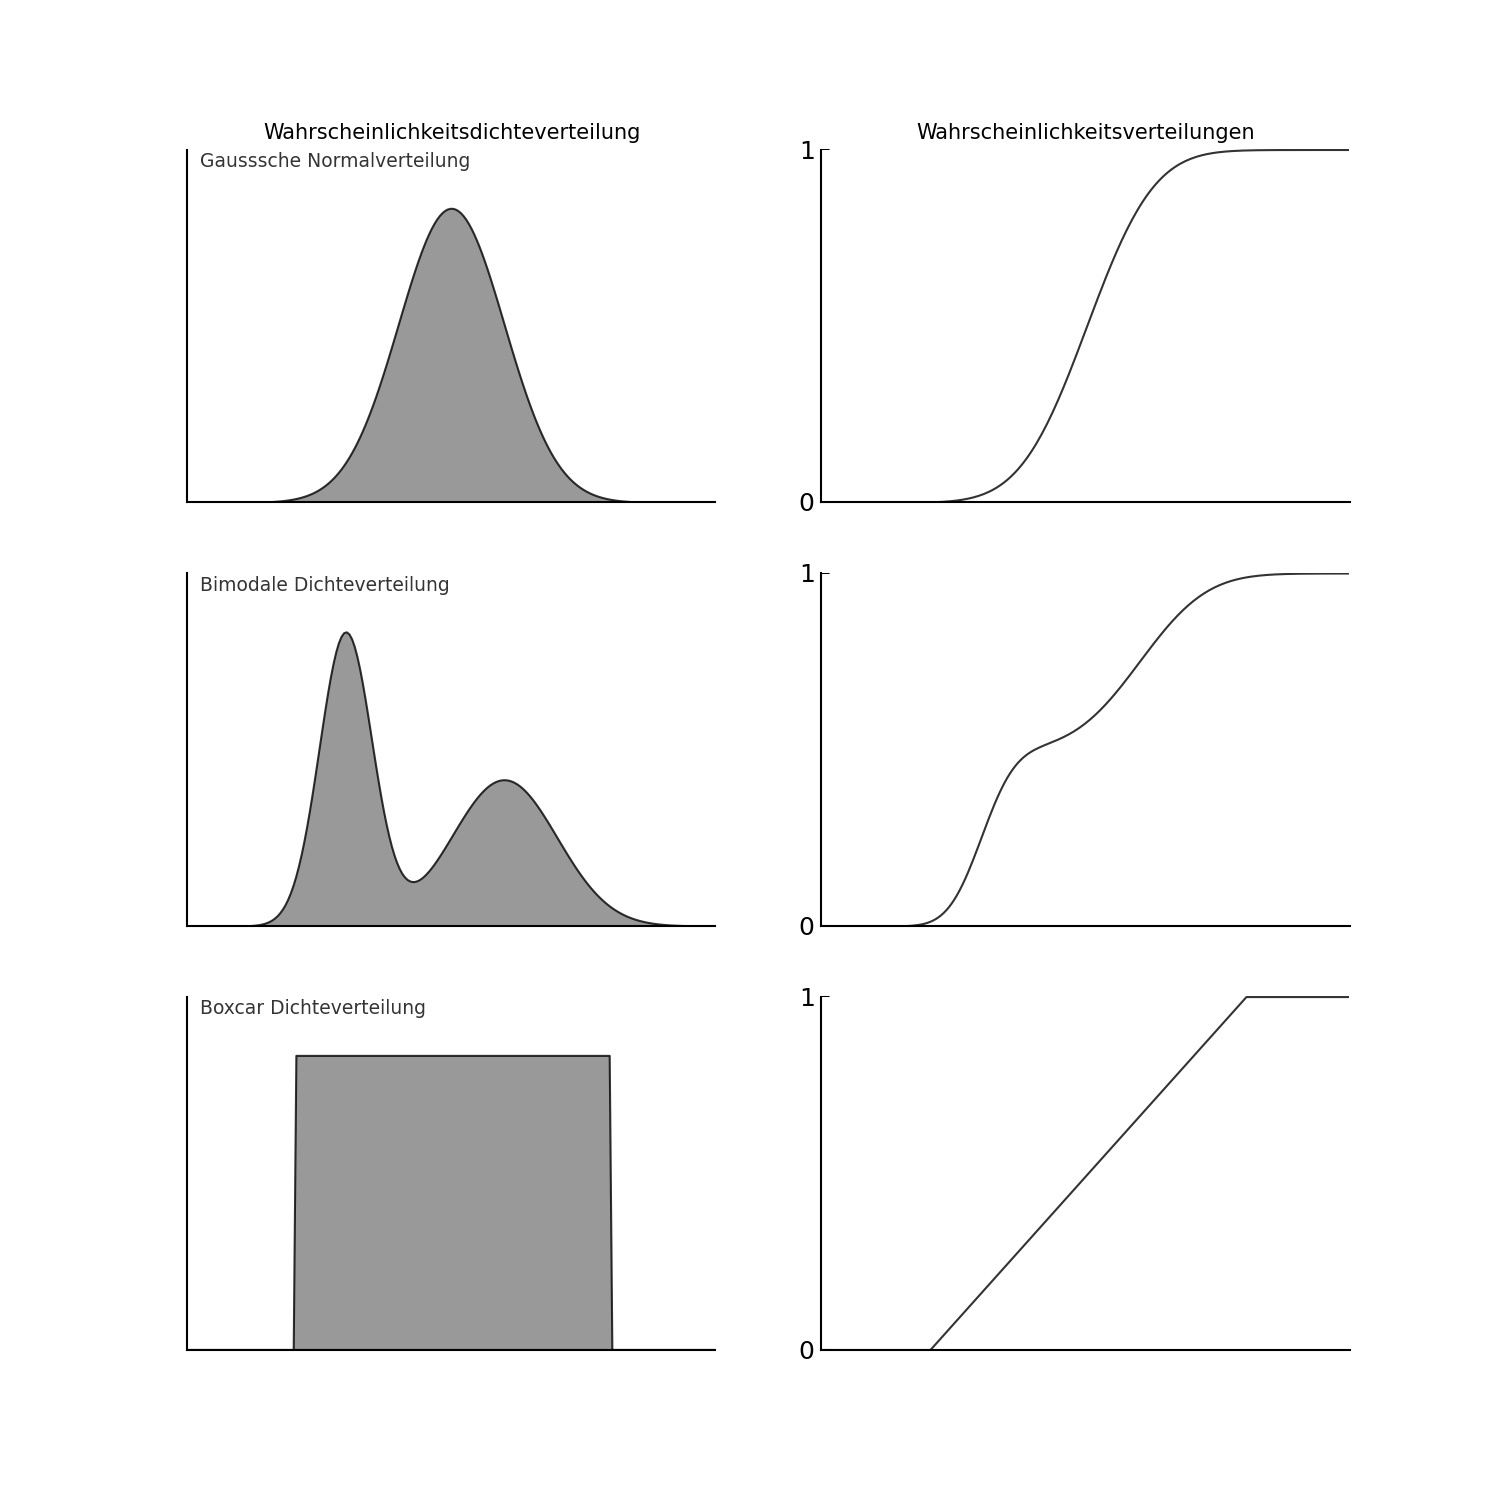
\includegraphics[width=1\tw]{fig/02-Definitionen/dichtefunktionen.png}
\caption{Verteilung verschiedene Wahrscheinlichkeitsdichtefunktionen (links) und die entsprechende Verteilungsfunktion (rechts). Von oben nach unten: Unimodale Gaussverteilung, Bimodale Gaussverteilung und die Gleichverteilung.}
\label{fig:stoch_distribution}
\end{figure}

\subsubsection*{Beispiel Gaußsche Normalverteilung}
Beispiel einer Gaußsche Normalverteilung mit dem Mittelwert $m$ und der Standardabweichung $\sigma$. Die Zufallsgröße $x$ nimmt mit $\sim$68\%-iger Wahrscheinlichkeit Werte zwischen $m \pm \sigma$ an. Mit $\sim$95\%-iger Wahrscheinlichkeit Werte zwischen $m \pm 2\sigma$.\\
Die Verteilungsdichtefunktion bei Gaußscher Normalverteilung lautet:
\begin{equation}
p(s)=\frac{1}{\sigma \sqrt{2\pi}}e^{-\frac{(s-m)^2}{2\sigma^2}}
\end{equation}
und die dazugehörige Verteilungsfunktion
\[
P(s)=\frac{1}{\sigma \sqrt{2\pi}}\int\limits_{-\infty}^s e^{{-\frac{(s'-m)^2}{2\sigma^2}}}ds'.
\]
Mit der Fehlerfunktion der Gaußschen Normalverteilung
\[
\mbox{erf}(x)=\frac{2}{\sqrt{\pi}}\int\limits_0^x e^{-x'^2}dx',
\]
folgt für die Verteilungsfunktion
\[
P(s) = \frac{1}{2}(\mbox{erf}\left(\frac{s-m}{\sqrt{2} \sigma}) + 1\right).
\]
Der Wertebereich der Fehlerfunktion ist $[-1,1]$ und der Wertebereich der Verteilungsfunktion ist wie immer $[0,1]$. Aufgrund der Symmetrie der Gaußschen Wahrscheinlichkeitsdichteverteilung gilt $P(m-s) = 1 - P(m+s)$.

\subsection{Erwartungswerte und Momente}
Eigenschaften von Zufallsgrößen können sehr einfach mit Hilfe des Erwartungswertes und statistischer Momente beschrieben werden. Der \textit{Erwarungswert}, $E[x]$, der Zufallsgröße $x$ ist gleichzeitig der Schwerpunkt der Wahrscheinlichkeitsdichtefunktion:
\begin{equation}
E[x] = \int\limits_{-\infty}^{\infty}sp(s)ds
\end{equation}

\subsubsection*{Erstes Moment}
Das erste Moment der Verteilungsdichtefunktion entspricht dem Erwartungswert und ist gleichzeitig der \textbf{Mittelwert}:
\[
E[x]=m=m_1
\]
Der Erwartungswert wird mit Hilfe der Wahrscheinlichkeitsdichtefunktion definiert. Im Falle realer Wertereihen ist diese meistens unbekannt. Daher muss der Mittelwert anhand von Messungen, bzw. Stichproben $x_i$ ($i=1,\dots, N,$), geschätzt werden. Der so aus den Messungen ermittelte Mittelwert ist eine Schätzung für den Erwartungswert:
\begin{equation}
\bar{x} = \hat{m_1} = \frac{1}{N}\sum \limits_{i=1}^N x_i.
\end{equation}
Dabei deutet das Dach ($\hat{m_1}$) an, dass es sich um eine Schätzung handelt, in diesem Fall des ersten Moments.\\\\
Für den Erwartungswert gelten einfache Annahmen:
\[
E[x_1+x_2]=E[x_1]+E[x_2],
\]
sowie
\[
E[a]=a.
\]
Falls $a$ eine deterministische Größe ist, nimmt man für eine Messgröße ein Modell an nachdem sie sich aus dem tatsächlichen Wert $a$ und zufälligem Rauschen $n_i$  zusammensetzt:
\[
x_i = a + n_i
\]
So ist gilt für den Erwartungwert von $x_i$:
\[
E[x_i] = a + E[n_i]
\]
Ist der Erwartungswert von $n_i$ ungleich Null, kann auch durch Mittelung über mehrere Messwerte der tatsächliche Wert der gesuchten Größe nicht erhalten werden.\\

Es handelt sich um eine \textit{erwartungstreue} Schätzung (eng. \textsl{unbiased}), wenn der Erwartunswert der Schätzung gleich der gesuchten Größe ist:
\[
E[\hat{m_1} ]= m_1
\]
Denn der Mittelwert ergibt sich aus.
\[
E[\hat{m_1}] =\frac{1}{N}\sum \limits_{i=1}^N E[x_i] = m_1
\]

Bei einer \textit{nicht erwartungstreue} Schätzung (eng. \textsl{biased}), benötigt man mehrere Messungen um die gesuchte Größe aus dem Mittelwert schätzen zu können:
\[
\lim\limits_{N \to \infty}\frac{1}{N}\sum \limits_{i=1}^N x_i=E[x]=m_1
\]
Dabei nimmt mit Anzahl der Messungen der Fehler der Messung ab.

\subsubsection*{Zweites Moment}
Das \textit{zweite Moment} wird auch \textbf{Varianz} genannt und ist ein Maß für die Streuung des Messerwerte in einer Messreihe:
\begin{equation}
E[x^2]= \int\limits_{-\infty}^{\infty} s^2 p(s) ds=m_2
\end{equation}
Aus einer abzählbaren Anzahl von Messungen kann der zweite Moment geschätzt werden:
\begin{equation}
\bar x^2 = \hat{m_2} = \frac{1}{N}\sum\limits_{i=1}^N x_i^2
\end{equation}
Ausgedrückt in Erwartungswerten zeigt sich
\[
\alpha_2 = E[(x-E[x])^2].
\]
Aus einer Messreiehe kann die Varianz der Messwerte bestimmt werden als
\begin{equation}
\mbox{Var} = \sigma^2=\frac{1}{N-1}\sum \limits_{i=1}^N (x_i - \bar x)^2.
\end{equation}
Dabei ist $\sigma$ die \textsl{Standardabweichung} der Wertereiehe.\\\\
Auch für eine Schätzung kann die Varianz angegeben werden:
\[
E[(\hat{m}-E[\hat{m}])^2]
\]
Für eine Gaußsche Zufallsgröße ist die Varianz für die Schätzung des Mittelwertes
\[
\bar x = \sigma^2/N.
\]
Die Standardabweichung der Schätzung des Mittelwertes (\textit{Standardfehler}) ist dann 
\[
\sigma/\sqrt{N}.
\]
Wenn die Verzerrung und die Varianz einer Schätzung gegen Null gehen und $N$ gegen Unendlich, handelt es sich um eine \textit{konsistente Schätzung}. Das ist im Fall der Schätzung des Mittelwertes der Fall.\\

\subsubsection*{Höhere Momente}
Es können auch \textit{höhere Momente} definiert werden. Das $n$-te Moment ist:
\[
m_n=E[x^n]
\]
Dieses kann mittels
\[
\hat{m_n}=\frac {1}{N} \sum\limits_{i=1}^N (x_i)^n
\]
geschätzt werden. 
Für das $n$-te \textit{zentrale höhere Moment} gilt der Erwartungswert:
\[
\alpha_n = E[(x-E[x])^n
\]
Die Schätzung des $n$-ten Moments aus einer diskreten Wertereihe ist definiert als:
\begin{equation}
\hat{\alpha_n}=\frac {1}{N-1} \sum_{i=1}^N (x_i - \bar x)^n
\end{equation}

Die Eigenschaften einer Zufallsgröße können auch durch die Gesamtheit der Momente eindeutig beschrieben werden. So beschreiben höherer Momente die \textbf{Schiefe} und die \textbf{Kurtosis}. Die Schiefe ($S$) ist ein Maß für die Asymetrie der Verteilungsdichtefunktion
\[
S = \frac {\alpha_3}{\sigma^3}=\frac {\alpha_3}{\alpha_2^{\frac{3}{2}}}
\]
und die Kurtosis ($K$) ein Maß für die Abweichung von der Gaußverteilung:
\[
K=\frac {\alpha_4}{\sigma^4}=\frac {\alpha_4}{\alpha_2^2}
\]
Die Kurtosis einer Gaußsche Zufallsverteilung beträgt 3.\\
Die Schiefe und Kurtosis können mit Hilfe der Schätzungen für die höheren zentralen Momente geschätzt werden:
\[
\hat S=\frac {\hat{\alpha_3}}{\hat{\alpha}_2^{\frac{3}{2}}},
\]
für die Schiefe, bzw. für die Kurtosis:
\[
\hat K=\frac {\hat{\alpha_4}}{\hat{\alpha_2^2}}
\]


\subsection{Stochastischer Prozess}

Eine Folge von Zufallsgrößen ${x_i}$ wird als stochastischer Prozess oder Zufallsprozess $\{x_i\}$ bezeichnet. Ein stochastischer Prozess kann auch eine kontinuierliche Funktion, z.B. der Zeit, sein: $x(t)$.\\\\
Dabei existiert für jeden Index $i$ bzw. jede Zeit $t$ eine Zufallsgröße, deren Eigenschaften durch Wahrscheinlichkeitsdichtefunktionen beschrieben werden. So kann z.B. für eine seismische Spur das Modell eines stochastischen Prozesses angenommen werden. Jede einzelne Spur (Messung) wird dann als Realisierung eines stochastischen Prozesses angesehen.\\
Im Folgenden wird die Realisierung des stochastischen Prozesses $\{x_i\}$ mit dem Index $j$ beschrieben:
\[
\{x_{ij}\} \mbox{ bzw. }  x_j(t).
\]
Gibt es mehrere Realisierungen spricht man auch von einem \textit{Ensemble}.\\\\
Der Erwartungswert eines stochastischen Prozesses kann mittels des Ensemble-Mittelwerts geschätzt werden, wenn die Anzahl der Realisierungen gegen Undendlich geht. Der Ensemble-Mittelwert von $x(t)$ für Zeit $t=t_1$ ist:
\[
\frac{1}{N}\sum\limits_{j=1}^{N}x_j(t_1)
\]
Es kann auch über die Zeit gemittelt werden. Das ergibt den Zeit-Mittelwert für die Realisierung $j$:
\[
\frac{1}{2T}\int\limits_{-T}^{T}x_j(t)dt
\]
Ensemble- und Zeit-Mittelwert müssen nicht, können aber, gleich sein. Vorraussetzung für die Gleichheit ist, dass der Erwartungswert eines stochastischen Prozesses zeitunabhängig ist. Man spricht von einem ergodischen Prozess oder \textit{Ergodizität}, wenn für $N \to \infty$ der Ensemble-Mittelwert gleich dem Zeit-Mittelwert ist. Sind alle Eigenschaften des stochastischen Prozesses zeitunabhängig, liegt (starke) \textbf{Stationalität} vor.\\\\
Sind alle Zufallsgrößen $x_i$ eine stochstischen Prozesses $\{x_i\}$ gaußverteilt, spricht man von einem {\bf Gaußprozess}. Im Fall eines Gaußschen iid-Prozesses (\textsl{independent and identicaly distributed process}) sind alle Zufallsgrößen unabhängig und identisch gaußverteilt.
Alle Zufallsgrößen eines iid-Prozesses sind unabhängig und identisch verteilt.

\newpage


\section{Signal-Rausch-Verhältnis}
Das Signal-Rausch-Verhältnis (eng. \textsl{Signal-To-Noise ratio}, SNR) dient der Einschätzung der Messqualität. Das SNR wird aus den Daten abgeschätzt. Zunächst wird ein Modell der Verteilung angenommen:
\[
x_i=s_i + n_i
\]
Dabei sind $x_i$ die untersuchte Wertereihe, $s_i$ das Nutzsignal und  $n_i$ ist störendes Rauschen. Weiterhin soll gelten $E[s_i]=E[n_i]=0$ und $max\{|s_i|\}=|s|_{max}$ bzw. $max\{|n_i|\}=|n|_{max}$.\\
In Abhängigkeit des Modells gibt es verschiedene Möglichkeiten für die Abschätzung des SNR. Dabei ist entscheidend, welche Komponenten als deterministisch bzw. stochastisch angenommen werden.
\begin {itemize}
\item $s_i$ und $n_i$ sind deterministisch:
\[
\mathrm{SNR} = \frac {|s|_{max}}{|n|_{max}}
\]
\item $s_i$ deterministisch, $n_i$ stochastisch (iid ZP, gleichverteilt):
\[
\mathrm{SNR} = \frac {|s|_{max}}{|n|_{max}}
\]
\item $s_i$ deterministisch, $n_i$ stochastisch (gaußverteilt):
\[
\mathrm{SNR} = \frac {|s|_{max}}{\sigma_n}
\]
\item $s_i$ stochastisch, $n_i$ stochastisch (iid ZP, gaußverteilt):
\[
\mathrm{SNR} = \frac {\sigma_s}{\sigma_n}
\]
\end{itemize}

Für die Schätzung von $|s|_{max}, \sigma_s$ bzw. $|n|_{max}, \sigma_n$ wird ein Zeitfenster ausgesucht, in dem für das Rauschen  $n_i\approx 0$ gilt (Signalfenster) bzw. ein Rauschfenster in dem $s_i \approx 0$ ist. Überlagern sich Rauschen und Signal zeitlich ständig, müssen weitergehende Analysen durchgeführt werden.


\section{Energie- und Leistungssignal}
Ein transientes Signal, d.h. ein Signal endlicher zeitlicher Länge, wird auch als Energiesignal bezeichnet.  Für die Energie gilt
\[
\int_a^b |s(t)|^2 dt < \infty
\]
Ein Leistungssignal besitzt eine unendliche zetliche Länge, d.h. es dauert länger an als Beobachtungsintervall lang ist. 
Es wird die Leistung in dem Zeitintervall $[a,b]$ bestimmt
\[
\frac{1}{b-a}\int\limits_a^b |s(t)|^2 dt.
\]
Dabei bedeutet der Faktor $\frac{1}{b-a}$ eine Mittelung über die Zeit.

